\subsection{Elementary Operations on Sets}

\newcommand\venndiagiii[7]{
    \begin{center}
        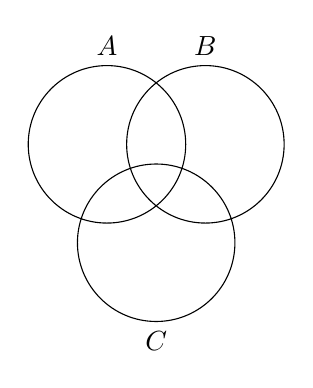
\begin{tikzpicture}[fill=gray]
            \def\bx{1.25}
            \def\cy{-1.25}
            \def\circA{(0,0) circle (1)}
            \def\circB{(\bx,0) circle (1)}
            \def\circC{(\bx/2,\cy) circle (1)}
            \def\vennrect{(-1,\cy-1) rectangle (\bx+1,1)}
            \def\@true{1}

            % A only
            \ifx1#1
                \begin{scope}
                    \clip \vennrect \circB;
                    \clip \vennrect \circC;
                    \fill \circA;
                \end{scope}
            \fi

            % B only
            \ifx1#2
                \begin{scope}
                    \clip \vennrect \circA;
                    \clip \vennrect \circC;
                    \fill \circB;
                \end{scope}
            \fi

            % C only
            \ifx1#3
                \begin{scope}
                    \clip \vennrect \circA;
                    \clip \vennrect \circB;
                    \fill \circC;
                \end{scope}
            \fi

            % A and B only
            \ifx1#4
                \begin{scope}
                    \clip \vennrect \circC;
                    \clip \circA;
                    \clip \circB;
                    \fill \circA;
                \end{scope}
            \fi

            % A and C only
            \ifx1#5
                \begin{scope}
                    \clip \vennrect \circB;
                    \clip \circA;
                    \clip \circC;
                    \fill \circA;
                \end{scope}
            \fi

            % B and C only
            \ifx1#6
                \begin{scope}
                    \clip \vennrect \circA;
                    \clip \circB;
                    \clip \circC;
                    \fill \circB;
                \end{scope}
            \fi

            % A and B and C
            \ifx1#7
                \begin{scope}
                    \clip \circA;
                    \clip \circB;
                    \clip \circC;
                    \fill \circA;
                \end{scope}
            \fi

            % Draw circles and labels
            \draw \circA (0,1)  node [text=black,above] {$A$}
            \circB (\bx,1)  node [text=black,above] {$B$}
            \circC (\bx/2,\cy-1)  node [text=black,below] {$C$};
        \end{tikzpicture}
    \end{center}
}
\newcommand\venndiagii[3]{
    \begin{center}
        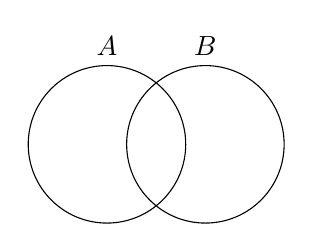
\begin{tikzpicture}[fill=gray]
            \def\bx{1.25}
            \def\circA{(0,0) circle (1)}
            \def\circB{(\bx,0) circle (1)}
            \def\vennrect{(-1,-1) rectangle (\bx+1,1)}
            \def\@true{1}

            % A only
            \ifx1#1
                \begin{scope}
                    \clip \vennrect \circB;
                    \fill \circA;
                \end{scope}
            \fi

            % B only
            \ifx1#2
                \begin{scope}
                    \clip \vennrect \circA;
                    \fill \circB;
                \end{scope}
            \fi

            % A and B only
            \ifx1#3
                \begin{scope}
                    \clip \circA;
                    \clip \circB;
                    \fill \circA;
                \end{scope}
            \fi

            % Draw circles and labels
            \draw \circA (0,1)  node [text=black,above] {$A$}
            \circB (\bx,1)  node [text=black,above] {$B$};
        \end{tikzpicture}
    \end{center}
}

\exercise{1}{
    Prove all the displayed formulas in this section and visualize them using Venn diagrams.
}
\sol{
    \newcommand*{\comproof}[2]{
        \ali{
            x \in A #1 B &\bic x \in A #2 x \in B \\
            &\bic x \in B #2 x \in A \\
            &\bic x \in B #1 A,
        }
    }
    \newcommand*{\assocproof}[2]{
        \ali{
            (A #1 B ) #1 C &\bic x \in A #1 B #2 x \in C \\
            &\bic (x \in A #2 x \in B) #2 x \in C \\
            &\bic x \in A #2 x \in B #2 x \in C \\
            &\bic x \in A #2 (x \in B #2 x \in C) \\
            &\bic x \in A #2 x \in B #1 C \\
            &\bic x \in A #1 (B #1 C),
        }
    }
    For commutivity, Venn diagrams are not very useful.
    \qproof{
        For all $x$, we have that
        \comproof{\cap}{\land}
        which shows that $A \cap B = B \cap A$.
        Similarly, we have that
        \comproof{\cup}{\lor}
        which proves that $A \cup B = B \cup A$.
    }

    Venn diagrams also provide no insight for associativity.
    \qproof{
        Again, for any $x$, we have that
        \assocproof{\cap}{\land}
        showing that $(A \cap B) \cap C = A \cap (B \cap C)$.
        Likewise, we have
        \assocproof{\cup}{\lor}
        and hence $(A \cup B) \cup C = A \cup (B \cup C)$.
    }

    \newcommand*{\distproof}[4]{
        \ali{
            x \in A #1 (B #2 C) &\bic x \in A #3 (x \in B #4 x \in C) \\
            &\bic (x \in A #3 x \in B) #4 (x \in A #3 x \in C) \\
            &\bic x \in A #1 B #4 x \in A #1 C \\
            &\bic x \in (A #1 B) #2 (A #1 C),
        }
    }
    For distributivity, Venn diagrams \emph{do} provide insight.
    The Venn diagram for the distributive identity $A \cap (B \cup C) = (A \cap B) \cup (A \cap C)$ is shown below:
    \venndiagiii{0}{0}{0}{1}{1}{0}{1}
    A proof of this follows directly from the distributivity of logical conjunction.
    \qproof{
        For all $x$, we have
        \distproof{\cap}{\cup}{\land}{\lor}
        which proves the result.
    }
    Likewise, the Venn diagram for $A \cup (B \cap C) = (A \cup B) \cap (A \cup C)$ is shown below:
    \venndiagiii{1}{0}{0}{1}{1}{1}{1}
    This time, the proof follows directly from the distributivity of logical disjunction.
    \qproof{
        For every $x$, we have that
        \distproof{\cup}{\cap}{\lor}{\land}
        proving the desired result.
    }

    \newcommand\demorgproof[4]{
        \ali{
            x \in C - (A #1 B) &\bic x \in C \land x \notin A #1 B \\
            &\bic x \in C \land \lnot (x \in A #1 B) \\
            &\bic x \in C \land \lnot (x \in A #2 x \in B) \\
            &\bic x \in C \land (x \notin A #3 x \notin B) \\
            &\bic (x \in C \land x \notin A) #3 (x \in C \land x \notin B) \\
            &\bic x \in C - A #3 x \in C - B \\
            &\bic x \in (C - A) #4 (C - B),
        }
    }
    Regarding the two DeMorgan laws, proofs of these rely on the DeMorgan and distributive laws of logic.
    First, we have $C - (A \cap B) = (C - A) \cup (C - B)$:
    \venndiagiii{0}{0}{1}{0}{1}{1}{0}
    \qproof{
        For all $x$,
        \demorgproof{\cap}{\land}{\lor}{\cup}
        of course showing the result.
    }
    The other DeMorgan law is of course $C - (A \cup B) = (C - A) \cap (C - B)$:
    \venndiagiii{0}{0}{1}{0}{0}{0}{0}
    \qproof{
        Again, for all $x$, we have
        \demorgproof{\cup}{\lor}{\land}{\cap}
        which proves the result.
    }

    Next, we have the property $A \cap (B - C) = (A \cap B) - C$, which is visualized below:
    \venndiagiii{0}{0}{0}{1}{0}{0}{0}
    The proof of this follows from the associativity of logical conjunction.
    \qproof{
        For all $x$, we have
        \ali{
            x \in A \cap (B - C) &\bic x \in A \land x \in B - C \\
            &\bic x \in A \land (x \in B \land x \notin C) \\
            &\bic (x \in A \land x \in B) \land x \notin C \\
            &\bic x \in A \cap B \land x \notin C \\
            &\bic x \in (A \cap B) - C,
        }
        showing the result.
    }

    The next claim is that $A - B = \es$ if and only if $A \ss B$, for which a Venn diagram is not useful.
    \qproof{
        \bicproof{
            First suppose that $A - B = \es$ and consider any $x \in A$.
            Suppose that $x \notin B$.
            Then we would have $x \in A$ but $x \notin B$ so that $x \in A - B$, contradicting the fact that $A - B = \es$.
            Hence, it has to be that $x \in B$ so that $A \ss B$ since $x$ was arbitrary.
        }{
            Now suppose that $A \ss B$ but that $A - B \neq \es$ so that there is an  $x \in A - B$.
            Therefore, $x \in A$ but $x \notin B$.
            However, since $A \ss B$ it must also be that $x \in B$ since $x \in A$, a contradiction!
            So it in fact has to be that $A - B = \es$ as desired.
        }
    }

    To prove the next property, it is first useful to establish the following lemma.
    \begin{lem}
        For any set $A$, $A - A = \es$.
    \end{lem}
    \qproof{
        This is very nearly self-evident, but suppose $A - A \neq \es$ so that there is an $x \in A - A$.
        Then it would both be true that $x \in A$ and $x \notin A$.
        As this is a clear contradiction, it has to be that in fact $A - A = \es$ as claimed.
    }
    The next property is then that $A \sd A = \es$, for which again a Venn diagram provides no insight and in fact does not really even make sense.
    \qproof{
        By definition and the above lemma,
        \gath{
            A \sd A = (A - A) \cup (A - A) = \es \cup \es = \es.
        }
        Clearly $\es \cup \es = \es$ since, were there an $x \in \es \cup \es$, we would have $x \in \es$ or $x \in \es$, the same impossibility in either case.
    }

    The penultimate property asserted in this section is that $A \sd B = B \sd A$.
    \qproof{
        This follows trivially from the commutativity of the union operation, proven above.
        By definition, we simply have
        \gath{
            A \sd B = (A - B) \cup (B - A) = (B - A) \cup (A - B) = B \sd A.
        }
    }

    The final property is $(A \sd B) \sd C = A \sd (B \sd C)$, i.e. that the symmetric difference operation is associative.
    This set is visualized below:
    \venndiagiii{1}{1}{1}{0}{0}{0}{1}
    In order to prove this while avoiding great tedium, we introduce the logical ``exclusive or'' operation, also called XOR.
    The reader may already have some familiarity with this operation, but for propositions $P$ and $Q$, we denote the XOR of $P$ and $Q$ as $P \lxor Q$.
    The XOR operation is defined by the following truth table:
    \begin{center}
        \begin{tabular}{cc|c}
            $P$ & $Q$ & $P \lxor Q$ \\
            \hline
            F   & F   & F           \\
            F   & T   & T           \\
            T   & F   & T           \\
            T   & T   & F
        \end{tabular}
    \end{center}
    \begin{lem}\label{lem:oper:xorid}
        We claim the logical identity $P \lxor Q \bic (P \land \lnot Q) \lor (Q \land \lnot P)$
    \end{lem}
    \qproof{
        To prove this, we work out the truth table for the right-hand side, in which we set $R = (P \land \lnot Q) \lor (Q \land \lnot P)$ for brevity:
        \begin{center}
            \begin{tabular}{cc|cc|cc|c}
                $P$ & $Q$ & $\lnot P$ & $\lnot Q$ & $P \land \lnot Q$ & $Q \land \lnot P$ & $R$ \\
                \hline
                F   & F   & T         & T         & F                 & F                 & F   \\
                F   & T   & T         & F         & F                 & T                 & T   \\
                T   & F   & F         & T         & T                 & F                 & T   \\
                T   & T   & F         & F         & F                 & F                 & F
            \end{tabular}
        \end{center}
        Since the truth table for $R$ is identical to that for $P \lxor Q$ above, this proves the identity.
    }
    \begin{lem}\label{lem:oper:xorassoc}
        The logical XOR operation is associative, that is that $(P \lxor Q) \lxor R \bic P \lxor (Q \lxor R)$.
    \end{lem}
    \qproof{
        This is again most easily proved via exhaustive truth tables:
        \begin{center}
            \begin{tabular}{ccc|c|c}
                $P$ & $Q$ & $R$ & $P \lxor Q$ & $(P \lxor Q) \lxor R$ \\
                \hline
                F   & F   & F   & F           & F                     \\
                F   & F   & T   & F           & T                     \\
                F   & T   & F   & T           & T                     \\
                F   & T   & T   & T           & F                     \\
                T   & F   & F   & T           & T                     \\
                T   & F   & T   & T           & F                     \\
                T   & T   & F   & F           & F                     \\
                T   & T   & T   & F           & T
            \end{tabular}
        \end{center}
        \pagebreak
        \begin{center}
            \begin{tabular}{ccc|c|c}
                $P$ & $Q$ & $R$ & $Q \lxor R$ & $P \lxor (Q \lxor R)$ \\
                \hline
                F   & F   & F   & F           & F                     \\
                F   & F   & T   & T           & T                     \\
                F   & T   & F   & T           & T                     \\
                F   & T   & T   & F           & F                     \\
                T   & F   & F   & F           & T                     \\
                T   & F   & T   & T           & F                     \\
                T   & T   & F   & T           & F                     \\
                T   & T   & T   & F           & T
            \end{tabular}
        \end{center}
        Since the final column of both tables are identical, this shows the desired result.
    }
    \begin{lem}\label{lem:oper:sdxor}
        For sets $A$ and $B$ and any $x$, $x \in A \sd B$ if and only if $x \in A \lxor x \in B$.
    \end{lem}
    \qproof{
        For any $x$, define the proposition $P$ as $x \in A$ and $Q$ as $x \in B$.
        Then we have that
        \ali{
            x \in A \sd B &\bic x \in (A -  B) \cup (B - A) & \text{Definition of $\sd$} \\
            &\bic x \in A - B \lor x \in B - A & \text{Definition of union} \\
            &\bic (x \in A \land x \notin B) \lor (x \in B \land x \notin A) & \text{Definition of set difference} \\
            &\bic (P \land \lnot Q) \lor (Q \land \lnot P) & \text{Definitions of $P$ and $Q$} \\
            &\bic P \lxor Q & \text{Lemma~\ref{lem:oper:xorid}} \\
            &\bic x \in A \lxor x \in B, & \text{Definitions of $P$ and $Q$}
        }
        which of course proves the result.
    }
    Finally, we are ready to prove the original assertion that the symmetric difference is associative.
    \qproof{
        For any $x$, define the proposition $P$ as $x \in A$, $Q$ as $x \in B$ and $R$ as $x \in C$.
        We then have that
        \ali{
            x \in (A \sd B) \sd C &\bic (x \in A \lxor x \in B) \lxor x \in C & \text{Lemma~\ref{lem:oper:sdxor}} \\
            &\bic (P \lxor Q) \lxor R & \text{Definitions of $P$, $Q$, and $R$} \\
            &\bic P \lxor (Q \lxor R) & \text{Lemma~\ref{lem:oper:xorassoc}} \\
            &\bic x \in A \lxor (x \in B \lxor x \in C) & \text{Definitions of $P$, $Q$, and $R$} \\
            &\bic x \in A \sd (B \sd C). & \text{Lemma~\ref{lem:oper:sdxor}}
        }
        This of course suffices to show that $(A \sd B) \sd C = A \sd (B \sd C)$.
    }
}

\exercise{2}{
    Prove:
    \begin{enumerate}
        \item[(a)] $A \ss B$ if and only if $A \cap B = A$ if and only if $A \cup B = B$ if and only if $A - B = \es$.
        \item[(b)] $A \ss B \cap C$ if and only if $A \ss B$ and $A \ss C$.
        \item[(c)] $B \cup C \ss A$ if and only if $B \ss A$ and $C \ss A$.
        \item[(d)] $A - B = (A \cup B) -B = A - (A \cap B)$.
        \item[(e)] $A \cap B = A - (A - B)$.
        \item[(f)] $A - (B - C) = (A - B) \cup (A \cap C)$.
        \item[(g)] $A = B$ if and only if $A \sd B = \es$.
    \end{enumerate}
}
\sol{
    (a) \qproof{
        \bicproof{
            First assume that $A \ss B$.

            To show that $A \cap B = A$, first consider $x \in A \cap B$, then clearly $x \in A$ so that $A \cap B \ss A$.
            Now suppose that $x \in A$ so that also $x \in B$ since $A \ss B$.
            Hence, $x \in A$ and $x \in B$ so that $x \in A \cap B$, showing that $A \ss A \cap B$.

            Next we show that $A \cup B = B$.
            First consider any $x \in A \cup B$.
            If $x \in A$ then also $x \in B$ since $A \ss B$.
            Since, in the other case, we have that $x \in B$ directly, it follows that $A \cup B \ss B$.
            Now suppose that $x \in B$ so that clearly also $x \in A \cup B$, and so $B \ss A \cup B$ as well.

            Finally, we show that $A - B = \es$.
            To see this, assume first that $A - B \neq \es$ so that there is an $x \in A - B$.
            Thus, $x \in A$ but $x \notin B$.
            However, $x \in A$ implies that $x \in B$ since $A \ss B$, which is a contradiction.
        }{
            First suppose that $A \cap B = A$ and consider any $x \in A$ so that also $x \in A \cap B$, and hence $x \in B$ as well.
            This shows that $A \ss B$.

            Next, suppose that $A \cup B = B$ and consider any $x \in A$.
            Then $x \in A \cup B = B$, which suffices to show that $x \in B$ and thus $A \ss B$.

            Lastly, suppose that $A - B = \es$ and consider any $x \in A$.
            Were it the case that $x \notin B$ then it would follow that $x \in A - B = \es$, an impossibility.
            Hence, it has to be that $x \in B$ as well so that $A \ss B$ again.
        }

        This all suffices to show that
        \gath{
            A \ss B \bic A \cap B = A \bic A \cup B = B \bic A - B = \es
        }
        as desired.
    }

    (b) \qproof{
        \bicproof{
            Suppose first that $A \ss B \cap C$ and consider any $x \in A$.
            Then also $x \in B \cap C$ so that both $x \in B$ and $x \in C$.
            As $x$ was arbitrary, this shows that both $A \ss B$ and $A \ss C$.
        }{
            Now suppose that $A \ss B$ and $A \ss C$ and consider any $x \in A$.
            Then both $x \in B$ since $A \ss B$, and $x \in C$ since $A \ss C$.
            Therefore, $x \in B \cap C$, showing that $A \ss B \cap C$.
        }
    }

    (c) \qproof{
        \bicproof{
            First suppose that $B \cup C \ss A$ and consider any $x \in B$.
            Then $x \in B \cup C$ so that also $x \in A$, showing that $B \ss A$.
            Similarly, for any $x \in C$ we have that again $x \in B \cup C$ so that $x \in A$.
            This shows that $C \ss A$ as well.
        }{
            Now suppose that both $B \ss A$ and $C \ss A$ and consider any $x \in B \cup C$.
            In the case in which $x \in B$, we have that $x \in A$ since $B \ss A$.
            In the other case in which $x \in C$ we also have $x \in A$ since $C \ss A$ as well.
            This shows that $B \cup C \ss A$ since $x$ was arbitrary.
        }
    }

    (d) \qproof{
        \seteqproof{
            Suppose that $x \in A - B$ so that $x \in A$ and $x \notin B$.
            Then of course also $x \in A \cup B$ since $x \in A$.
            Since also $x \notin B$ it follows that $x \in (A \cup B) - B$, showing that $A - B \ss (A \cup B) - B$.
            We also have that $x \notin A \cap B$ since $x \notin B$.
            Hence, also $x \in A - (A \cap B)$ so that $A - B \ss A - (A \cap B)$ as well.
        }{
            Suppose that $x \in (A \cup B) - B$.
            Then $x \in A \cup B$ and $x \notin B$.
            Since it must be that $x \in A$ or $x \in B$, but $x \notin B$, it must be that $x \in A$.
            Hence, $x \in A - B$, which proves that $(A \cup B) - B \ss A - B$.

            Now suppose that $x \in A - (A \cap B)$ so that $x \in A$ and $x \notin A \cap B$.
            Since $x \in A$ it has to be that $x \notin B$ since otherwise it would be that $x \in A \cap B$.
            Therefore, $x \in A$ and $x \notin B$ so that $x \in A - B$, showing that also $A - (A \cap B) \ss A - B$.

            This all is sufficient to show that
            \gath{
                A - B = (A \cup B) - B = A - (A \cap B)
            }
            as desired.
        }
    }

    (e) First, a somewhat obvious lemma.
    \begin{lem}\label{lem:oper:negsd}
        For any $x$, $x$ is \emph{not} a member of $A - B$ if and only if $x \notin A$ or $x \in B$.
    \end{lem}
    \qproof{
        This is shown with some basic rules of logic.
        For any $x$, we have
        \ali{
            x \notin A - B &\bic \lnot(x \in A - B) & \\
            &\bic \lnot(x \in A \land x \notin B) & \text{Definition of set difference} \\
            &\bic x \notin \lor x \in B, & \text{DeMorgan law for logical conjunction}
        }
        and it is as simple as that.
    }
    Now we can prove the desired result.
    \qproof{
        Consider any $x$.
        Let $F$ be the proposition that $x \in A$ and $x \notin A$, which is of course \emph{always} false.
        We then have
        \ali{
            x \in A \cap B &\bic x \in A \land x \in B & \text{Definition of set intersection} \\
            &\bic F \lor (x \in A \land x \in B) & \text{Since $F$ is always false} \\
            &\bic (x \in A \land x \notin A) \lor (x \in A \land x \in B) & \text{Definition of $F$} \\
            &\bic x \in A \land (x \notin A \lor x \in B) & \text{Distributive law for conjunction} \\
            &\bic x \in A \land x \notin A - B & \text{Lemma~\ref{lem:oper:negsd}} \\
            &\bic x \in A - (A - B), & \text{Definition of set difference}
        }
        showing the desired result.
    }

    (f) \qproof{
        Here we have, for any $x$,
        \ali{
            x \in A - (B - C) &\bic x \in A \land x \notin B - C & \text{Definition of set difference} \\
            &\bic x \in A \land (x \notin B \lor x \in C) & \text{Lemma~\ref{lem:oper:negsd}} \\
            &\bic (x \in A \land x \notin B) \lor (x \in A \land X \in C) & \text{Distributive law for conjunction} \\
            &\bic x \in A - B \lor x \in A \cap C & \text{Definitions of $-$ and $\cap$} \\
            &\bic x \in (A - B) \cup (A \cap C), & \text{Definition of set union}
        }
        which proves the result.
    }

    (g) \qproof{
        \bicproof{
            Suppose that $A = B$.
            Then $A \sd B = A \sd A = \es$ by a property of the symmetric difference that was listed in the text and proven in Exercise~1.4.1 above.
        }{
            Now suppose that $A \sd B = \es$.
            Then it follows that both $A - B = \es$ and $B - A = \es$ since otherwise we would have that $A \sd B = (A - B) \cup (B - A) \neq \es$.

            Now consider any $x \in A$ so that of course $x \notin A - B = \es$.
            Then, by Lemma~\ref{lem:oper:negsd}, we have that $x \notin A$ or $x \in B$.
            Hence, $x \in B$ since we have already established that $x \in A$.
            This shows that $A \ss B$.

            Now consider any $x \in B$ so that, similarly, $x \notin B - A = \es$.
            Then, again by Lemma~\ref{lem:oper:negsd}, $x \notin B$ or $x \in A$ so that $x \in A$ since $x \in B$.
            This shows that $B \ss A$ as well, and therefore that $A = B$ as desired.
        }
    }
}

\exercise{3}{
    For each of the following (false) statements draw a Venn diagram in which it fails:
    \begin{enumerate}
        \item[(a)] $A - B = B - A$.
        \item[(b)] $A \cap B \pss A$.
        \item[(c)] $A \ss B \cup C$ implies $A \ss B$ or $A \ss C$.
        \item[(d)] $B \cap C \ss A$ implies $B \ss A$ or $C \ss A$.
    \end{enumerate}
}
\sol{
    (a) The following is an arrangement of $A$ and $B$ the demonstrates the falsehood:
    \venndiagii{0}{0}{0}
    In particular, $A - B$ is
    \venndiagii{1}{0}{0}
    while $B - A$ is
    \venndiagii{0}{1}{0}
    which are clearly not equal.

    (b) This is demonstrated by the following sets:
    \begin{center}
        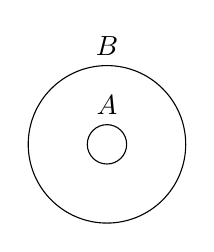
\begin{tikzpicture}
            \draw (0,0) circle (1) (0,1)  node [text=black,above] {$B$};
            \draw (0,0) circle (0.25) (0,0.25)  node [text=black,above] {$A$};
        \end{tikzpicture}
    \end{center}
    Here $A \ss B$ so that $A \cap B = A$, and hence $A \cap B$ is not a \emph{proper} subset of $A$.

    (c) Sets that contradict this assertion are shown below, in which $A$ is shaded:
    \begin{center}
        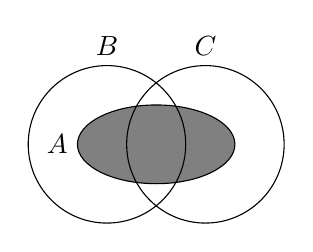
\begin{tikzpicture}
            \def\cx{1.25}
            \draw[fill=gray] (\cx/2,0) ellipse (1 and 0.5) (\cx/2-1,0) node [text=black,left] {$A$};
            \draw (0,0) circle (1) (0,1)  node [text=black,above] {$B$};
            \draw (\cx,0) circle (1) (\cx,1)  node [text=black,above] {$C$};
        \end{tikzpicture}
    \end{center}
    Here clearly $A$ is a subset of $B$ and $C$ taken together (i.e. $B \cup C$), but also clearly is a subset of neither $B$ nor $C$ alone.

    (d) Here is an example of sets that contradict this assertion, in which $B \cap C$ is shaded:
    \begin{center}
        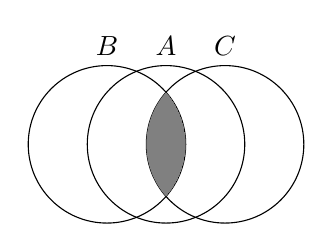
\begin{tikzpicture}[fill=gray]
            \def\cx{1.5}
            \def\circB{(0,0) circle (1)}
            \def\circC{(\cx,0) circle (1) (\cx,1)}
            \draw \circB (0,1)  node [text=black,above] {$B$};
            \draw \circC  node [text=black,above] {$C$};
            \draw (\cx/2,0) circle (1) (\cx/2,1) node [text=black,above] {$A$};

            % Shade B cap C
            \begin{scope}
                \clip \circB;
                \clip \circC;
                \fill \circB;
            \end{scope}
        \end{tikzpicture}
    \end{center}
    Clearly $B \cap C$ is a subset of $A$, but neither B not C alone are subsets of $A$.
}

\exercise{4}{
    Let $A$ be a set; show that a ``complement'' of $A$ does not exist.
    (The ``complement'' of $A$ is the set of all $x \notin A$.)
}
\sol{
    TODO
}

\exercise{5}{
    Let $S \neq \es$ and $A$ be sets.
    \begin{enumerate}
        \item[(a)] Set $T_1 = \braces{Y \in \pset{A} \where \text{$Y = A \cap X$ for some $X \in S$}}$, and prove $A \cap \bigcup S = \bigcup T_1$ (generalized distributive law).
        \item[(b)] Set $T_2 = \braces{Y \in \pset{A} \where \text{$Y = A - X$ for some $X \in S$}}$, and prove
            \gath{
                A - \bigcup S = \bigcap T_2 \\
                A - \bigcap S = \bigcup T_2
            }
            (generalized De Morgan's laws).
    \end{enumerate}
}
\sol{
    TODO
}

\exercise{6}{
    Prove that $\bigcap S$ exists for all $S \neq \es$.
    Where s the assumption that $S \neq \es$ used in the proof?
}
\sol{
    TODO
}